\documentclass[14pt]{beamer}
\mode<presentation>

\usepackage{graphicx}
\usepackage{geometry}
\usepackage{amsmath}
\usepackage{enumerate}
\usepackage{natbib}

\newcommand{\bone}{\mathbf{1}}
\newcommand{\bphi}{\boldsymbol{\phi}}
\newcommand{\sD}{\mathcal{D}}
\newcommand{\bm}{\mathbf{m}}
\newcommand{\bC}{\mathbf{C}}
\newcommand{\bA}{\mathbf{A}}
\newcommand{\btheta}{\boldsymbol{\theta}}
\newcommand{\bF}{\mathbf{F}}
\newcommand{\bG}{\mathbf{G}}
\newcommand{\bW}{\mathbf{W}}
\newcommand{\ba}{\mathbf{a}}
\newcommand{\bR}{\mathbf{R}}

\title{West \& Harrison \\ Chapter 10, Problem 7}
\author{The Dans}
\date{Thursday, March 16, 2017}

\begin{document}
	\maketitle
	
	\begin{frame}{The Data}
		The quarterly sales and cost index of a confectionary product are given as
		\begin{center}
			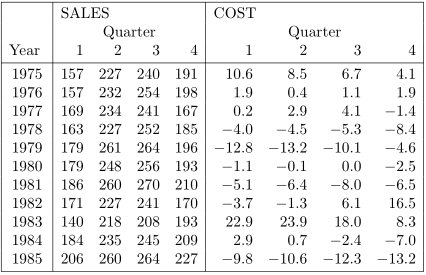
\includegraphics[width=0.5\linewidth]{Data}
		\end{center}
	\end{frame}

	\begin{frame}{The Goal}
		Fit a DLM to the sales with first-order polynomial, regression on cost, and full seasonal components. Based on previous information:
		{\footnotesize \begin{itemize}
			\item the underlying level of the series when cost is zero is 220 with a nominal standard error of 15
			\item the regression coefficient of cost is estimated as -1.5 with a standard error of about 0.7
			\item the seasonal factors for the four quarters of the first year are expected to be -50, 25, 50, -25, with nominal standard errors of 25, 15, 25, and 15, respectively
			\item the trend, regression, and seasonal components are initially assumed to be uncorrelated
			\item the observational variance is estimated as 100, with initial degrees of freedom of 12
		\end{itemize}}
	\end{frame}
	
	\begin{frame}{Part A}
		\textbf{Derive the appropriate initial prior that satisfies the zero-sum constraint.}
		
			\textit{Theorem 8.2: Imposing the constraint $\bone'\bphi = 0$ \\ on the prior $(\bphi_0|\sD_0^*) \sim \text{N}(\bm_0^*,\bC_0^*)$ \\ and writing $U = \bone'\bC_0^*\bone$ and $\bA = \bC_0^*\bone/U$ \\ gives the revised joint prior}	
		\begin{align*}
		(\bphi_0|\sD_0) & \sim \text{N}(\bm_0,\bC_0),\\
		\bm_0 = \bm_0^* & - \bA\bone'\bm_0^*,\\
		\bC_0 = \bC_0^* & - \bA\bA'U.
		\end{align*} 
	\end{frame}
	
	\begin{frame}{Part A}
		The given information on the seasonal components is
		\begin{align*}
		\bm_0^* & = (-25,-50,25,50)' &
		\bC_0^* & = \begin{pmatrix}
		225 & 0 & 0 & 0 \\
		0 & 625 & 0 & 0 \\
		0 & 0 & 225 & 0 \\
		0 & 0 & 0 & 625
		\end{pmatrix}.
		\end{align*}
		Remember to shift the seasonal components back one quarter, as time $t=0$ is the fourth quarter of 1974!
	\end{frame}

	\begin{frame}{Part A}
		Applying Theorem 8.2 yields
		\begin{align*}
		U & = 1700 \\ \bA & = (0.1323529, 0.3676471, 0.1323529, 0.3676471)' \\
		\bm_0^s & = (-25,-50,25,50)' \\
		\bC_0^s & = \begin{pmatrix}
		195.22 & -82.72 & -29.78 & -82.72 \\ 
		-82.72 & 395.22 & -82.72 & -229.78 \\ 
		-29.78 & -82.72 & 195.22 & -82.72 \\ 
		-82.72 & -229.78 & -82.72 & 395.22 
		\end{pmatrix}.
		\end{align*}
		The superscript $s$ denotes that this is for the seasonal component of the model.
	\end{frame}

	\begin{frame}{Part A}
		Therefore, the entire initial prior is
			{\footnotesize \begin{align*}
		\bm_0 & = (220,-1.5, -25, -50,  25,  50)' \\
		\bC_0 & = \begin{pmatrix}
		225.00 & 0.00 & 0.00 & 0.00 & 0.00 & 0.00 \\ 
		0.00 & 0.49 & 0.00 & 0.00 & 0.00 & 0.00 \\ 
		0.00 & 0.00 & 195.22 & -82.72 & -29.78 & -82.72 \\ 
		0.00 & 0.00 & -82.72 & 395.22 & -82.72 & -229.78 \\ 
		0.00 & 0.00 & -29.78 & -82.72 & 195.22 & -82.72 \\ 
		0.00 & 0.00 & -82.72 & -229.78 & -82.72 & 395.22 \\ 
		\end{pmatrix}.
		\end{align*}}
	\end{frame}

	\begin{frame}{Part B}
		\textbf{Identify the full initial prior quantities for the 6-dimensional state vector $\btheta_1$ and the observational variance $V$. Write down the defining quantities $\ba_1,\bR_1,n_0$, and $S_0$ based on the above initial information.}
	\end{frame}

	\begin{frame}{Part B}
		The DLM model in this case is defined as $\{ \bF_t, \bG,V,\bW_t \}$, with 
		\begin{align*}
		\bF_t & = (1,\text{Cost}_t,1,0,0,0)' &
		\bG & = \begin{pmatrix}
		1 & 0 & 0 & 0 & 0 & 0 \\
		0 & 1 & 0 & 0 & 0 & 0 \\
		0 & 0 & 0 & 1 & 0 & 0 \\
		0 & 0 & 0 & 0 & 1 & 0 \\
		0 & 0 & 0 & 0 & 0 & 1 \\
		0 & 0 & 1 & 0 & 0 & 0 \\
		\end{pmatrix}.
		\end{align*}
	\end{frame}

	\begin{frame}{Part B}
		
		{\scriptsize \begin{align*}
		\ba_1 & = \bG\bm_0 = (220,  -1.5,  25,  50, -25, -50)' \\
		\bR_1 & = \bG\bC_0\bG' + \bW_t = \begin{pmatrix}
		225.00 & 0.00 & 0.00 & 0.00 & 0.00 & 0.00 \\ 
		0.00 & 0.49 & 0.00 & 0.00 & 0.00 & 0.00 \\ 
		0.00 & 0.00 & 395.22 & -82.72 & -229.78 & -82.72 \\ 
		0.00 & 0.00 & -82.72 & 195.22 & -82.72 & -29.78 \\ 
		0.00 & 0.00 & -229.78 & -82.72 & 395.22 & -82.72 \\ 
		0.00 & 0.00 & -82.72 & -29.78 & -82.72 & 195.22 \\ 
		\end{pmatrix}  + \bW_t\\
		n_0 & = 12 \\
		S_0 & = 100.
		\end{align*}}
		Therefore, $(\btheta_1|\sD_0) \sim \text{T}_{6}(\ba_1,\bR_1)$ and $(V|\sD_0) \sim \text{Inverse Gamma}(n_0/2,d_0/2)$, where $d_0 = n_0S_0 = 1200$.
	\end{frame}

	\begin{frame}{Part C}
		\textbf{Use three discount factors to structure the evolution matrices of the model: $\delta_T$ for the constant intercept term, $\delta_R$ for the regression coefficient, and $\delta_S$ for the seasonal factors. Consider initially the values $\delta_T = \delta_S = 0.9$ and $\delta_R = 0.98$. Fit the model and perform the retrospective, filtering calculations to obtain filtered estimates of the state vector and all model components over time.}
	\end{frame}

	\begin{frame}{Part C}
		\begin{figure}
			\centering
			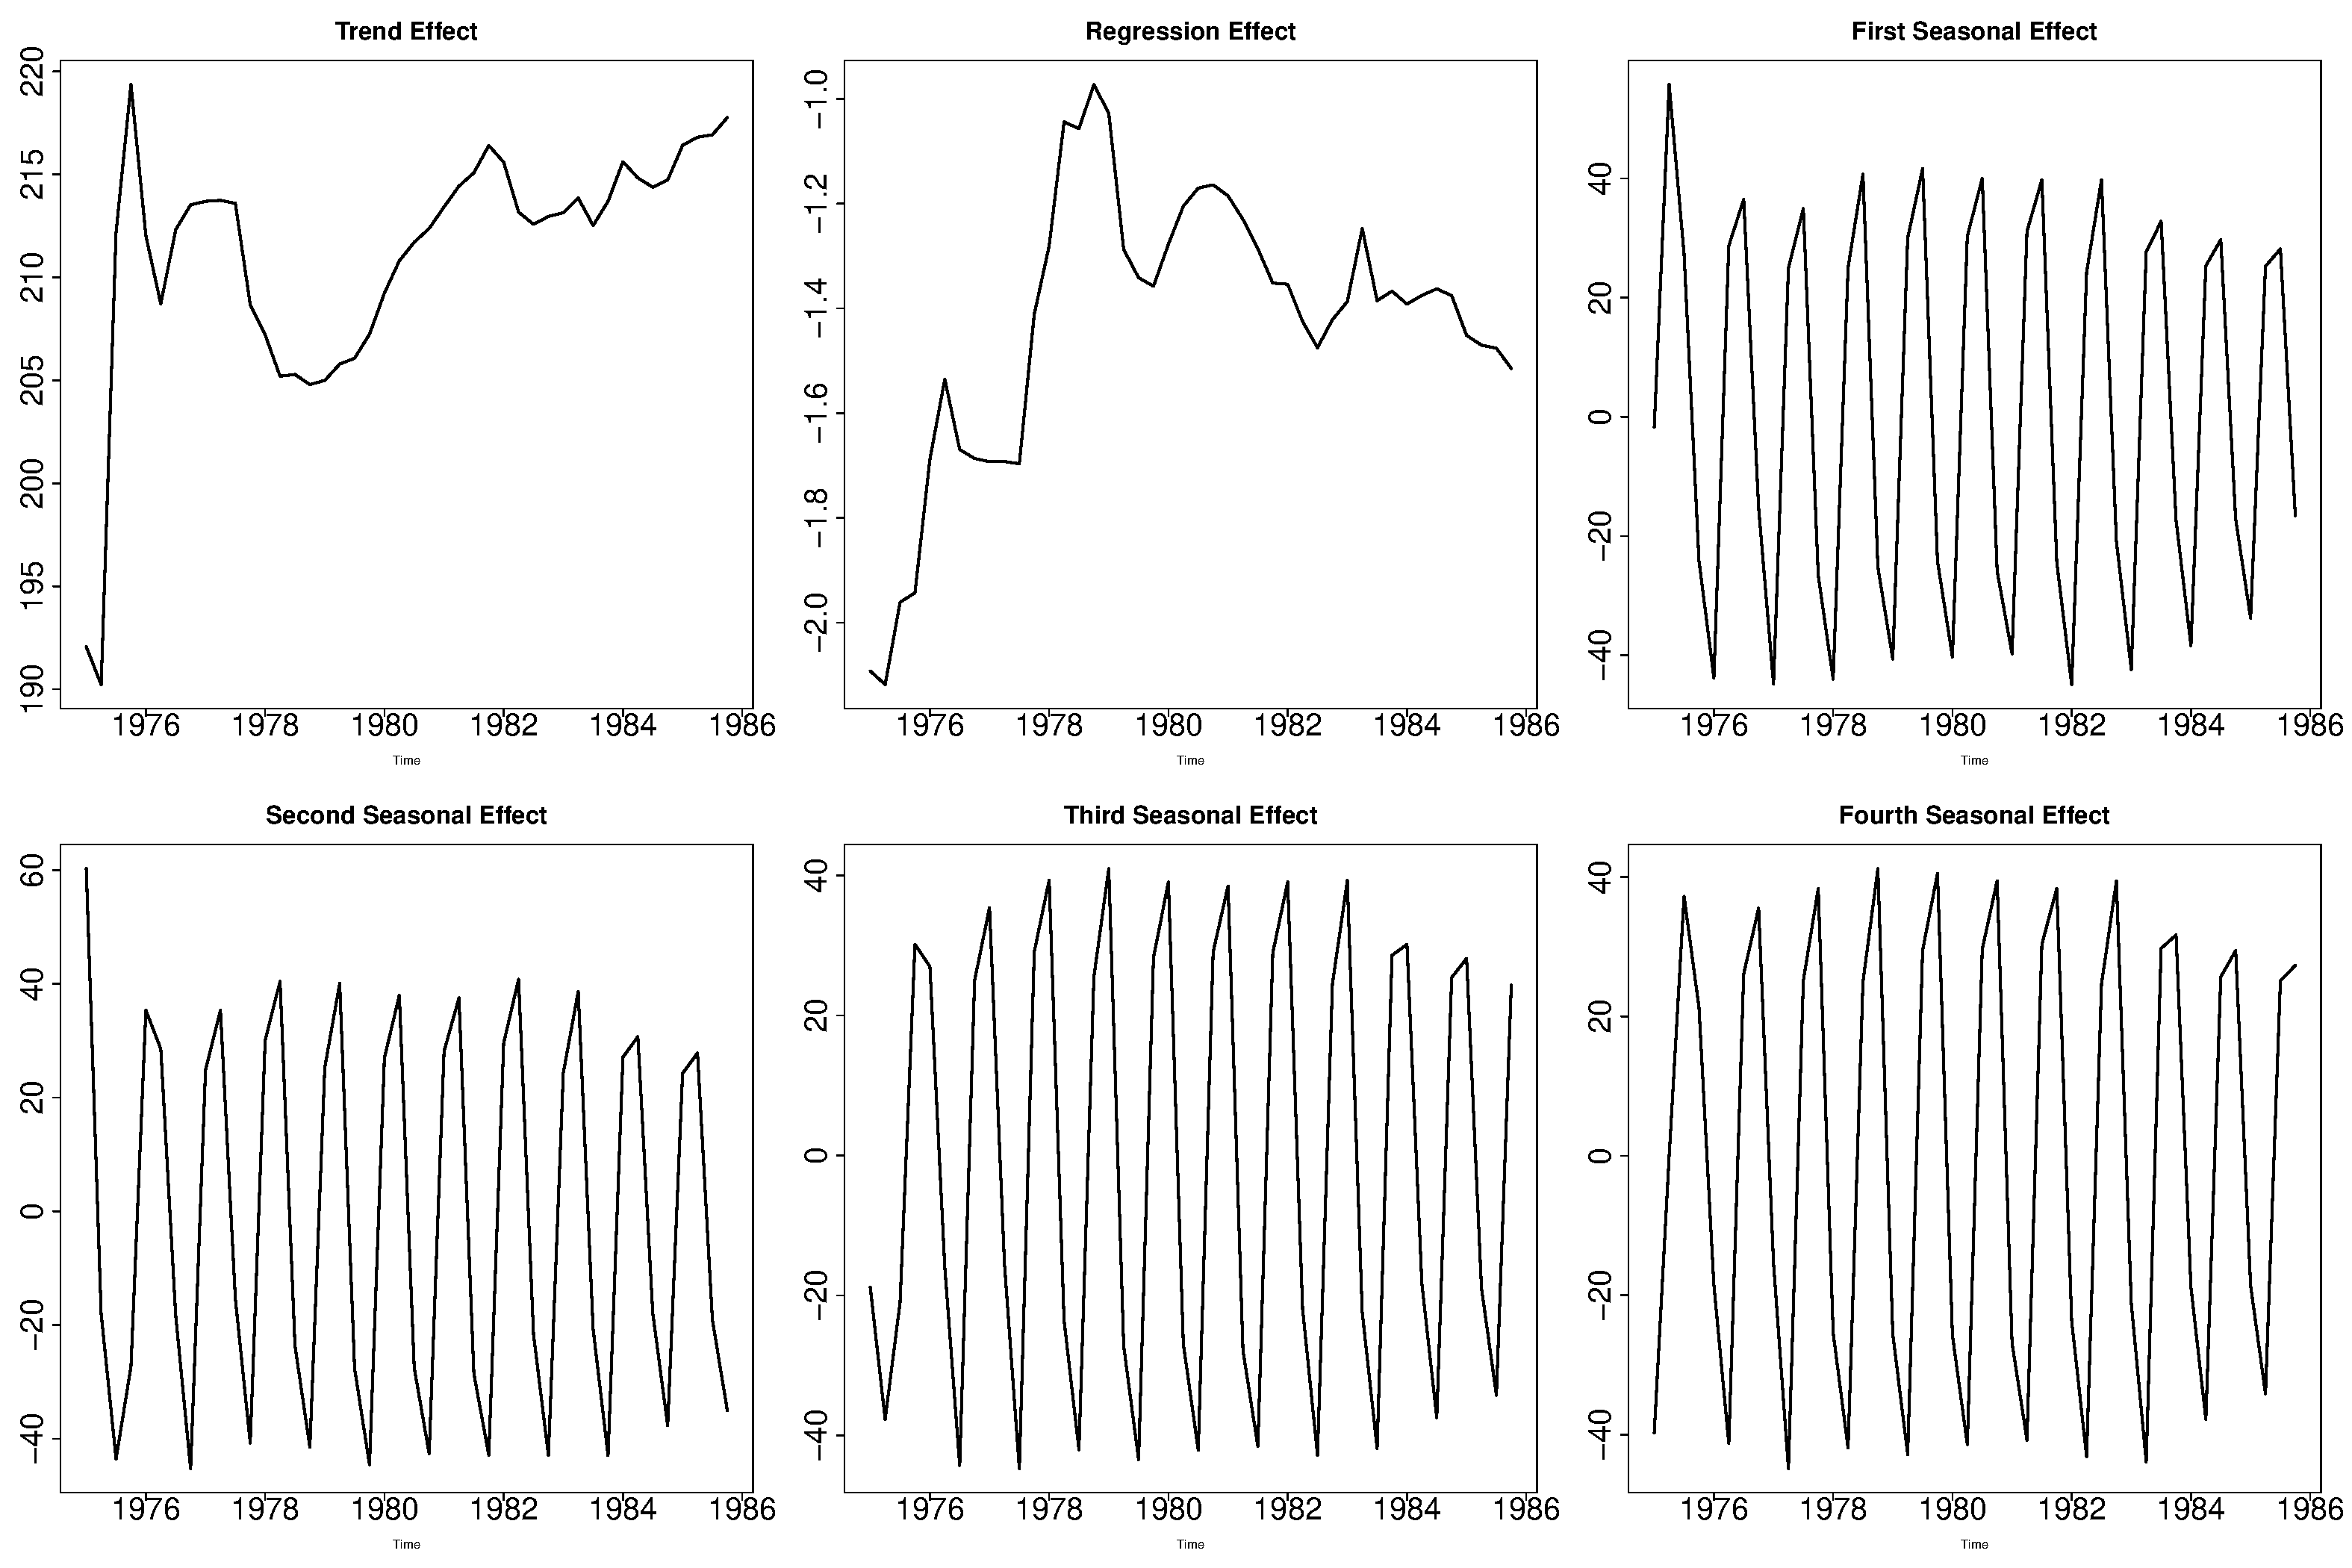
\includegraphics[width=\linewidth]{Filteredestimates}
			\caption{{\footnotesize Filtered estimates for all components of the state vector}}
			\label{fig:filteredestimates}
		\end{figure}
	\end{frame}

	\begin{frame}{Part C}
		\begin{figure}
			\centering
			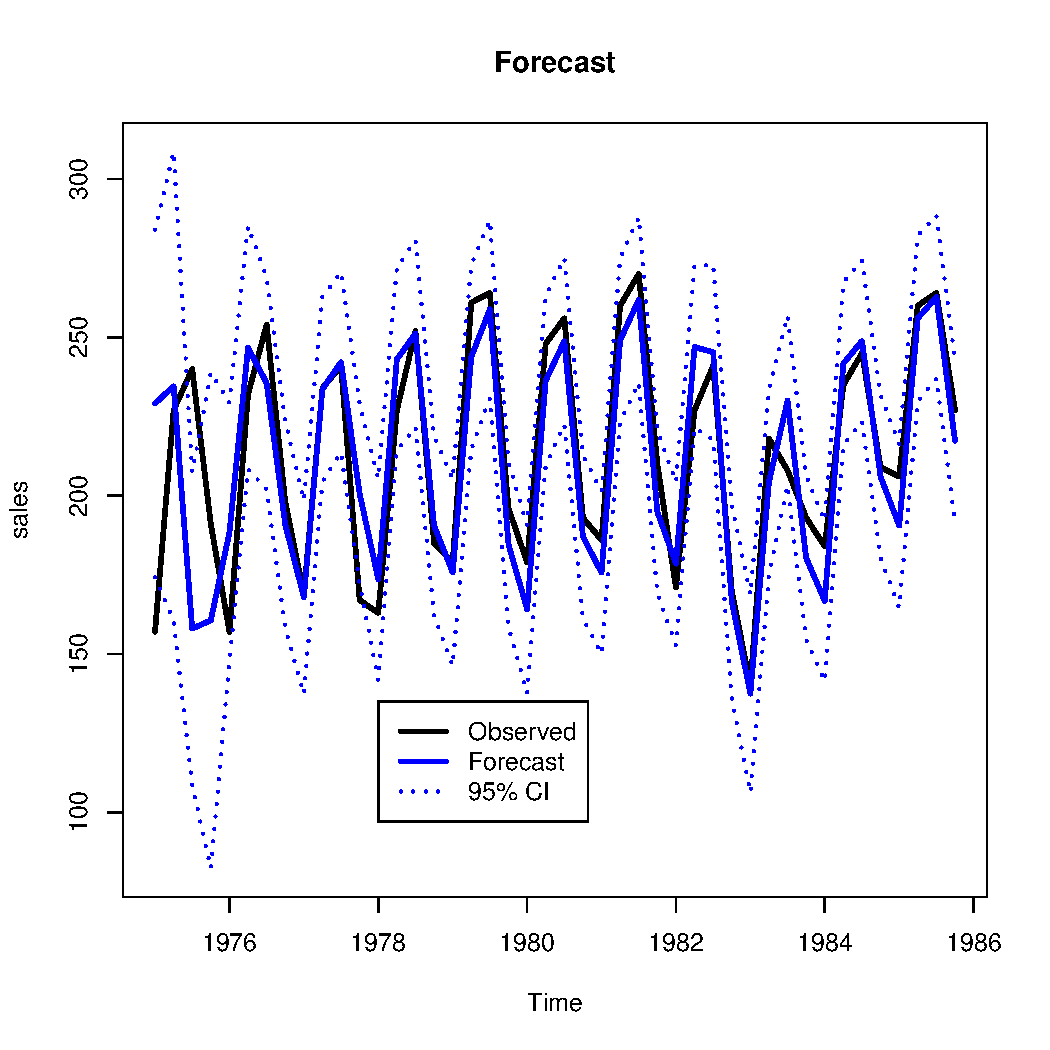
\includegraphics[width=0.65\linewidth]{ForecastDist}
			\caption{{\footnotesize One-step ahead forecast estimate and 95\% confidence interval}}
			\label{fig:forecastdist}
		\end{figure}
	\end{frame}

	\begin{frame}{Part D}
		\textbf{Based on this analysis, verify that the regression parameter on Cost is, in retrospect, rather stable over time.}
	\end{frame}

	\begin{frame}{Part D}
		\begin{figure}
			\centering
			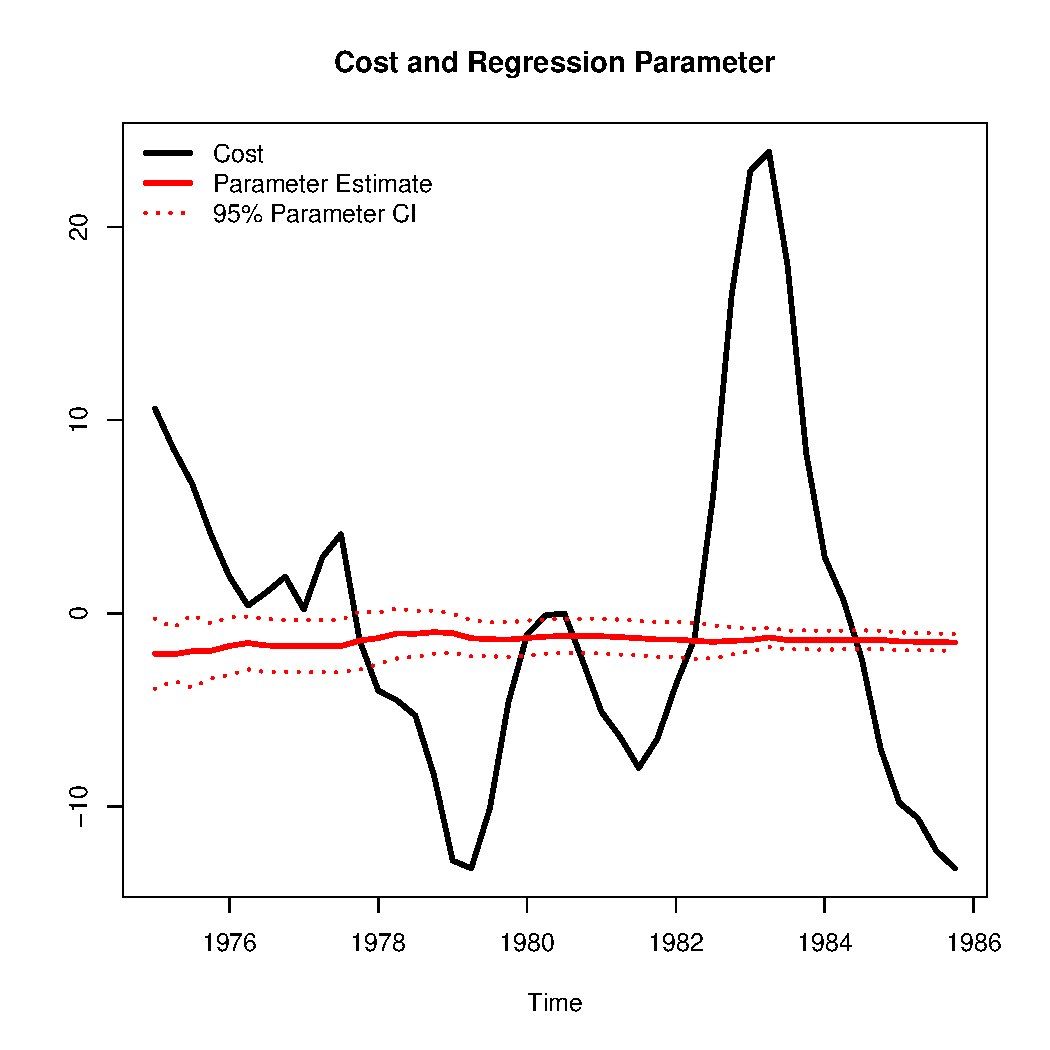
\includegraphics[width=0.65\linewidth]{CostandRegressionParm}
			%\caption{Plot of the observed cost and a summary of the distribution of the regression parameter}
			%\label{fig:costandregressionparm}
		\end{figure}
	\end{frame}

	\begin{frame}{Part D}
		\begin{figure}
			\centering
			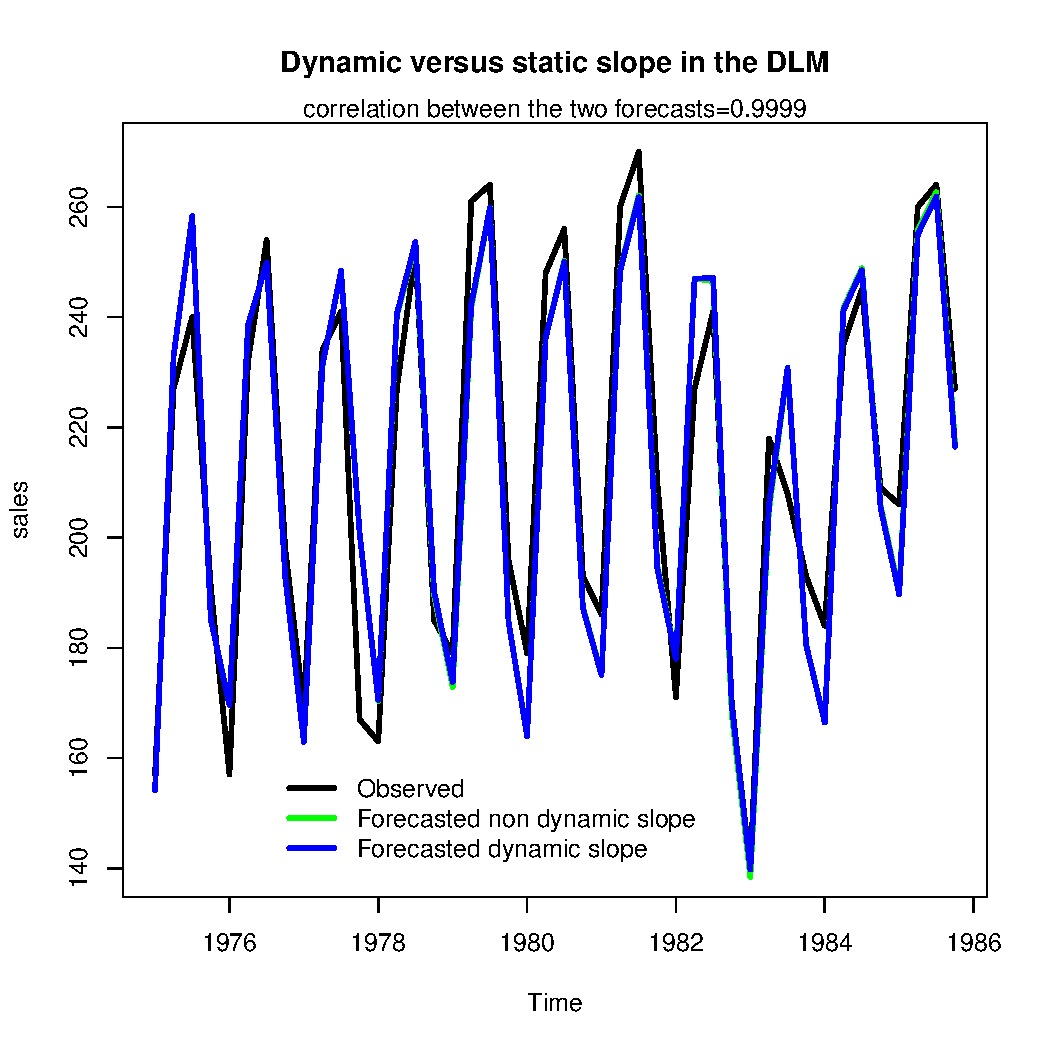
\includegraphics[width=0.7\linewidth]{DynVsStaticSlope}
%			\caption{Plot of the forecasts using a dynamic slope (blue) and a nondynamic slope (green)}
%			\label{fig:dynvsstatic}
		\end{figure}
	\end{frame}

	\begin{frame}{Part E}
		\textbf{Produce step ahead forecasts from the end of the data in the fourth quarter of 1985 for the next three years. The estimated values of Cost to be used in forecasting ahead are given by}
		\begin{center}
			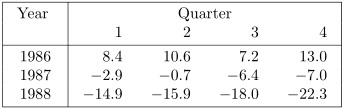
\includegraphics[width=0.5\linewidth]{CostFuture}
		\end{center}
	\end{frame}

	\begin{frame}{Part E}
		Appealing to \cite{harrison1999bayesian} page 199, and with $\bF(k)$ as the $\bF$ vector at time $k$, the $k$-step forecast distributions are
		{\footnotesize \begin{align*}
			(y(k)|\sD_T) & \sim T_{38}(F_T(k),Q_T(k))   \\
			F_T(k) & = \bF(k)'\ba_T(k) \\ Q_T(k) & = \bF(k)'\bR_T(k) \bF(k) \\
			\ba_T(k) & = \bG\ba_T(k-1)  \\ \bR_T(k) & = \bG\bR_T(k-1)\bG' \text{diag}\left( \frac{1}{\delta_t^k},\frac{1}{\delta_r^k},\frac{1}{\delta_s^k},\frac{1}{\delta_s^k},\frac{1}{\delta_s^k},\frac{1}{\delta_s^k} \right) 
		\end{align*}}
	\end{frame}

	\begin{frame}{Part E}
		\begin{figure}
			\centering
			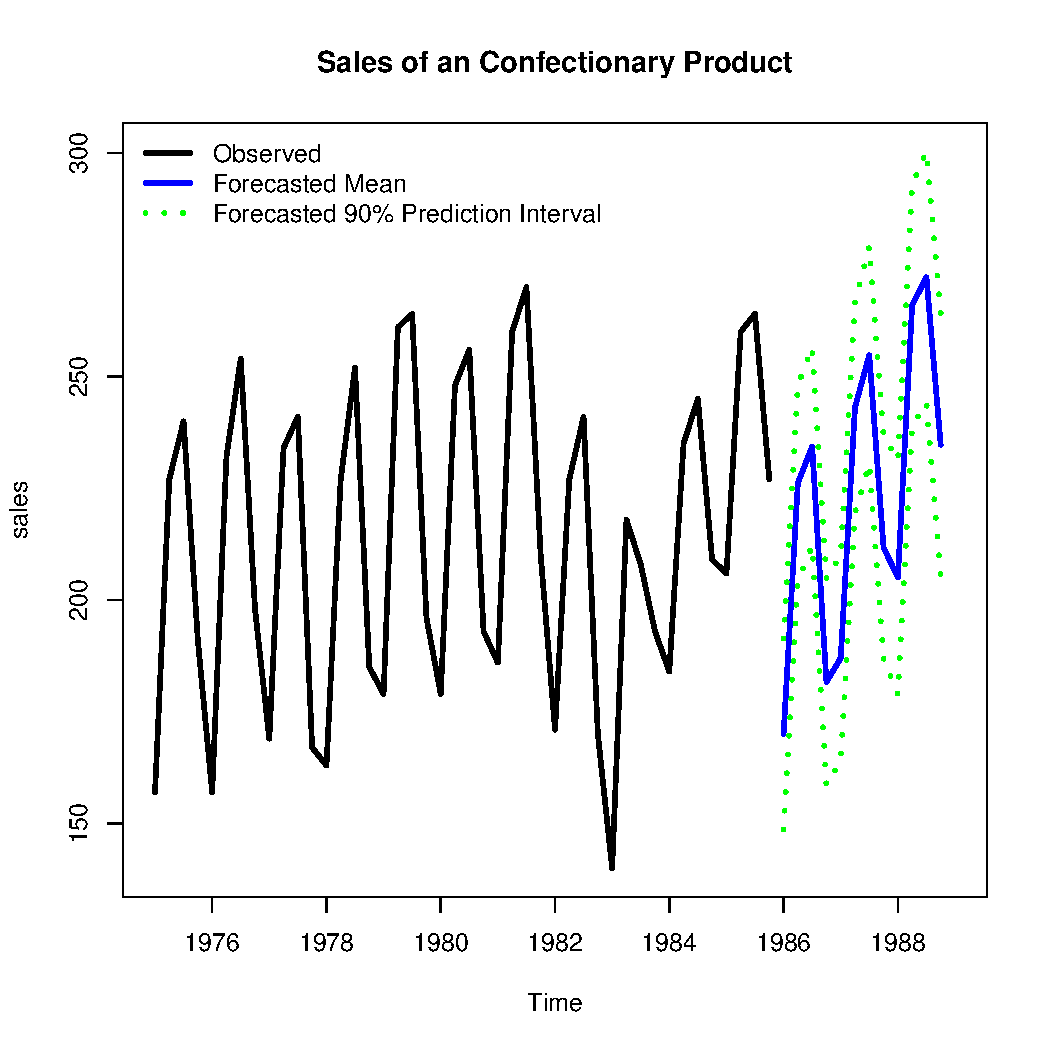
\includegraphics[width=0.7\linewidth]{StepAhead}
%			\caption{Step ahead forecasts for 1986 - 1988}
%			\label{fig:stepahead}
		\end{figure}
	\end{frame}

	\begin{frame}{References}
		\nocite{prado2010time}
%		\nocite{harrison1999bayesian}
		\bibliography{WHCh10Pr7}
		\bibliographystyle{plainnat}
	\end{frame}
	
\end{document}